\documentclass{article}
\usepackage{graphicx}
\usepackage{geometry}
\usepackage{enumitem}
\usepackage{hyperref}
\geometry{a4paper, margin=1in}


\title{Lab Report: Arduino Uno-Based Clock, Stopwatch, and Timer System}
\author{Dhawal \\ ee24btech11015}

\begin{document}

\maketitle

\section{Aim}
To design and implement a multifunctional display system using Arduino Uno that integrates:
\begin{itemize}
    \item Digital clock (with date/day display)
    \item Stopwatch (single-button control)
    \item Countdown timer (single-button control)
\end{itemize}
using 7-segment displays, LCD, and only 3 control buttons.

\section{Materials Required}
\subsection{Hardware Components}
\begin{itemize}
    \item Arduino Uno
    \item Six common cathode 7-segment displays
    \item 7447 BCD to 7-segment decoder IC
    \item 16×2 LCD
    \item Three push buttons
    \item 220 ohm resistors (for current limiting)
    \item 10k ohm resistors (for pull-up)
    \item Breadboard and jumper wires
    \item Potentiometer (for LCD contrast adjustment)
\end{itemize}

\subsection{Software}
\begin{itemize}
    \item Arduino IDE (for C++ code)
    \item AVR GCC (for C code)
\end{itemize}

\section{Circuit Connections}

\subsection{Seven-Segment Displays with 7447 IC}
\begin{itemize}
    \item \textbf{7447 IC Connections}:
    \begin{itemize}
        \item Pins A, B, C, D (BCD inputs) to Arduino Pins D2, D3, D4, D5
        \item Outputs (a, b, c, d, e, f, g) to All seven-segment displays (parallel connection)
    \end{itemize}
    \item \textbf{Common Cathode Control}:
    \begin{itemize}
        \item Each display's common cathode to Arduino Pins D6-D11 (via 220 ohm resistors)
    \end{itemize}
\end{itemize}

\subsection{16×2 LCD Connections}
\begin{itemize}
    \item \textbf{Control Pins}:
    \begin{itemize}
        \item RS → D12
        \item E → D13
        \item RW → GND
    \end{itemize}
    \item \textbf{Data Pins}:
    \begin{itemize}
        \item D4 → A0
        \item D5 → A1
        \item D6 → A2
        \item D7 → A3
    \end{itemize}
    \item \textbf{Contrast Adjustment}:
    \begin{itemize}
        \item V0 → Potentiometer middle pin
    \end{itemize}
\end{itemize}

\subsection{Button Connections (3-Button System)}
\begin{itemize}
    \item \textbf{Button 1 (Clock Mode)} to A4 (PC4)
    \item \textbf{Button 2 (Stopwatch)} to A5 (PC5)
    \begin{itemize}
        \item Single press: Resets and starts stopwatch
    \end{itemize}
    \item \textbf{Button 3 (Timer)} to D1 (PD1)
    \begin{itemize}
        \item Single press: Resets to preset value and starts countdown
    \end{itemize}
    \item All buttons use internal pull-up resistors
\end{itemize}

\subsection{Power Supply}
\begin{itemize}
    \item Arduino 5V to Power rail
    \item Arduino GND to Ground rail
\end{itemize}

\section{Observations}

\subsection{Clock Mode}
\begin{itemize}
    \item \textbf{Functionality}:
    \begin{itemize}
        \item 7-segment displays show time in HH:MM:SS format
        \item LCD shows date (DD/MM/YYYY) and blinking day indicator
    \end{itemize}
    \item \textbf{Image}:
    \begin{center}
        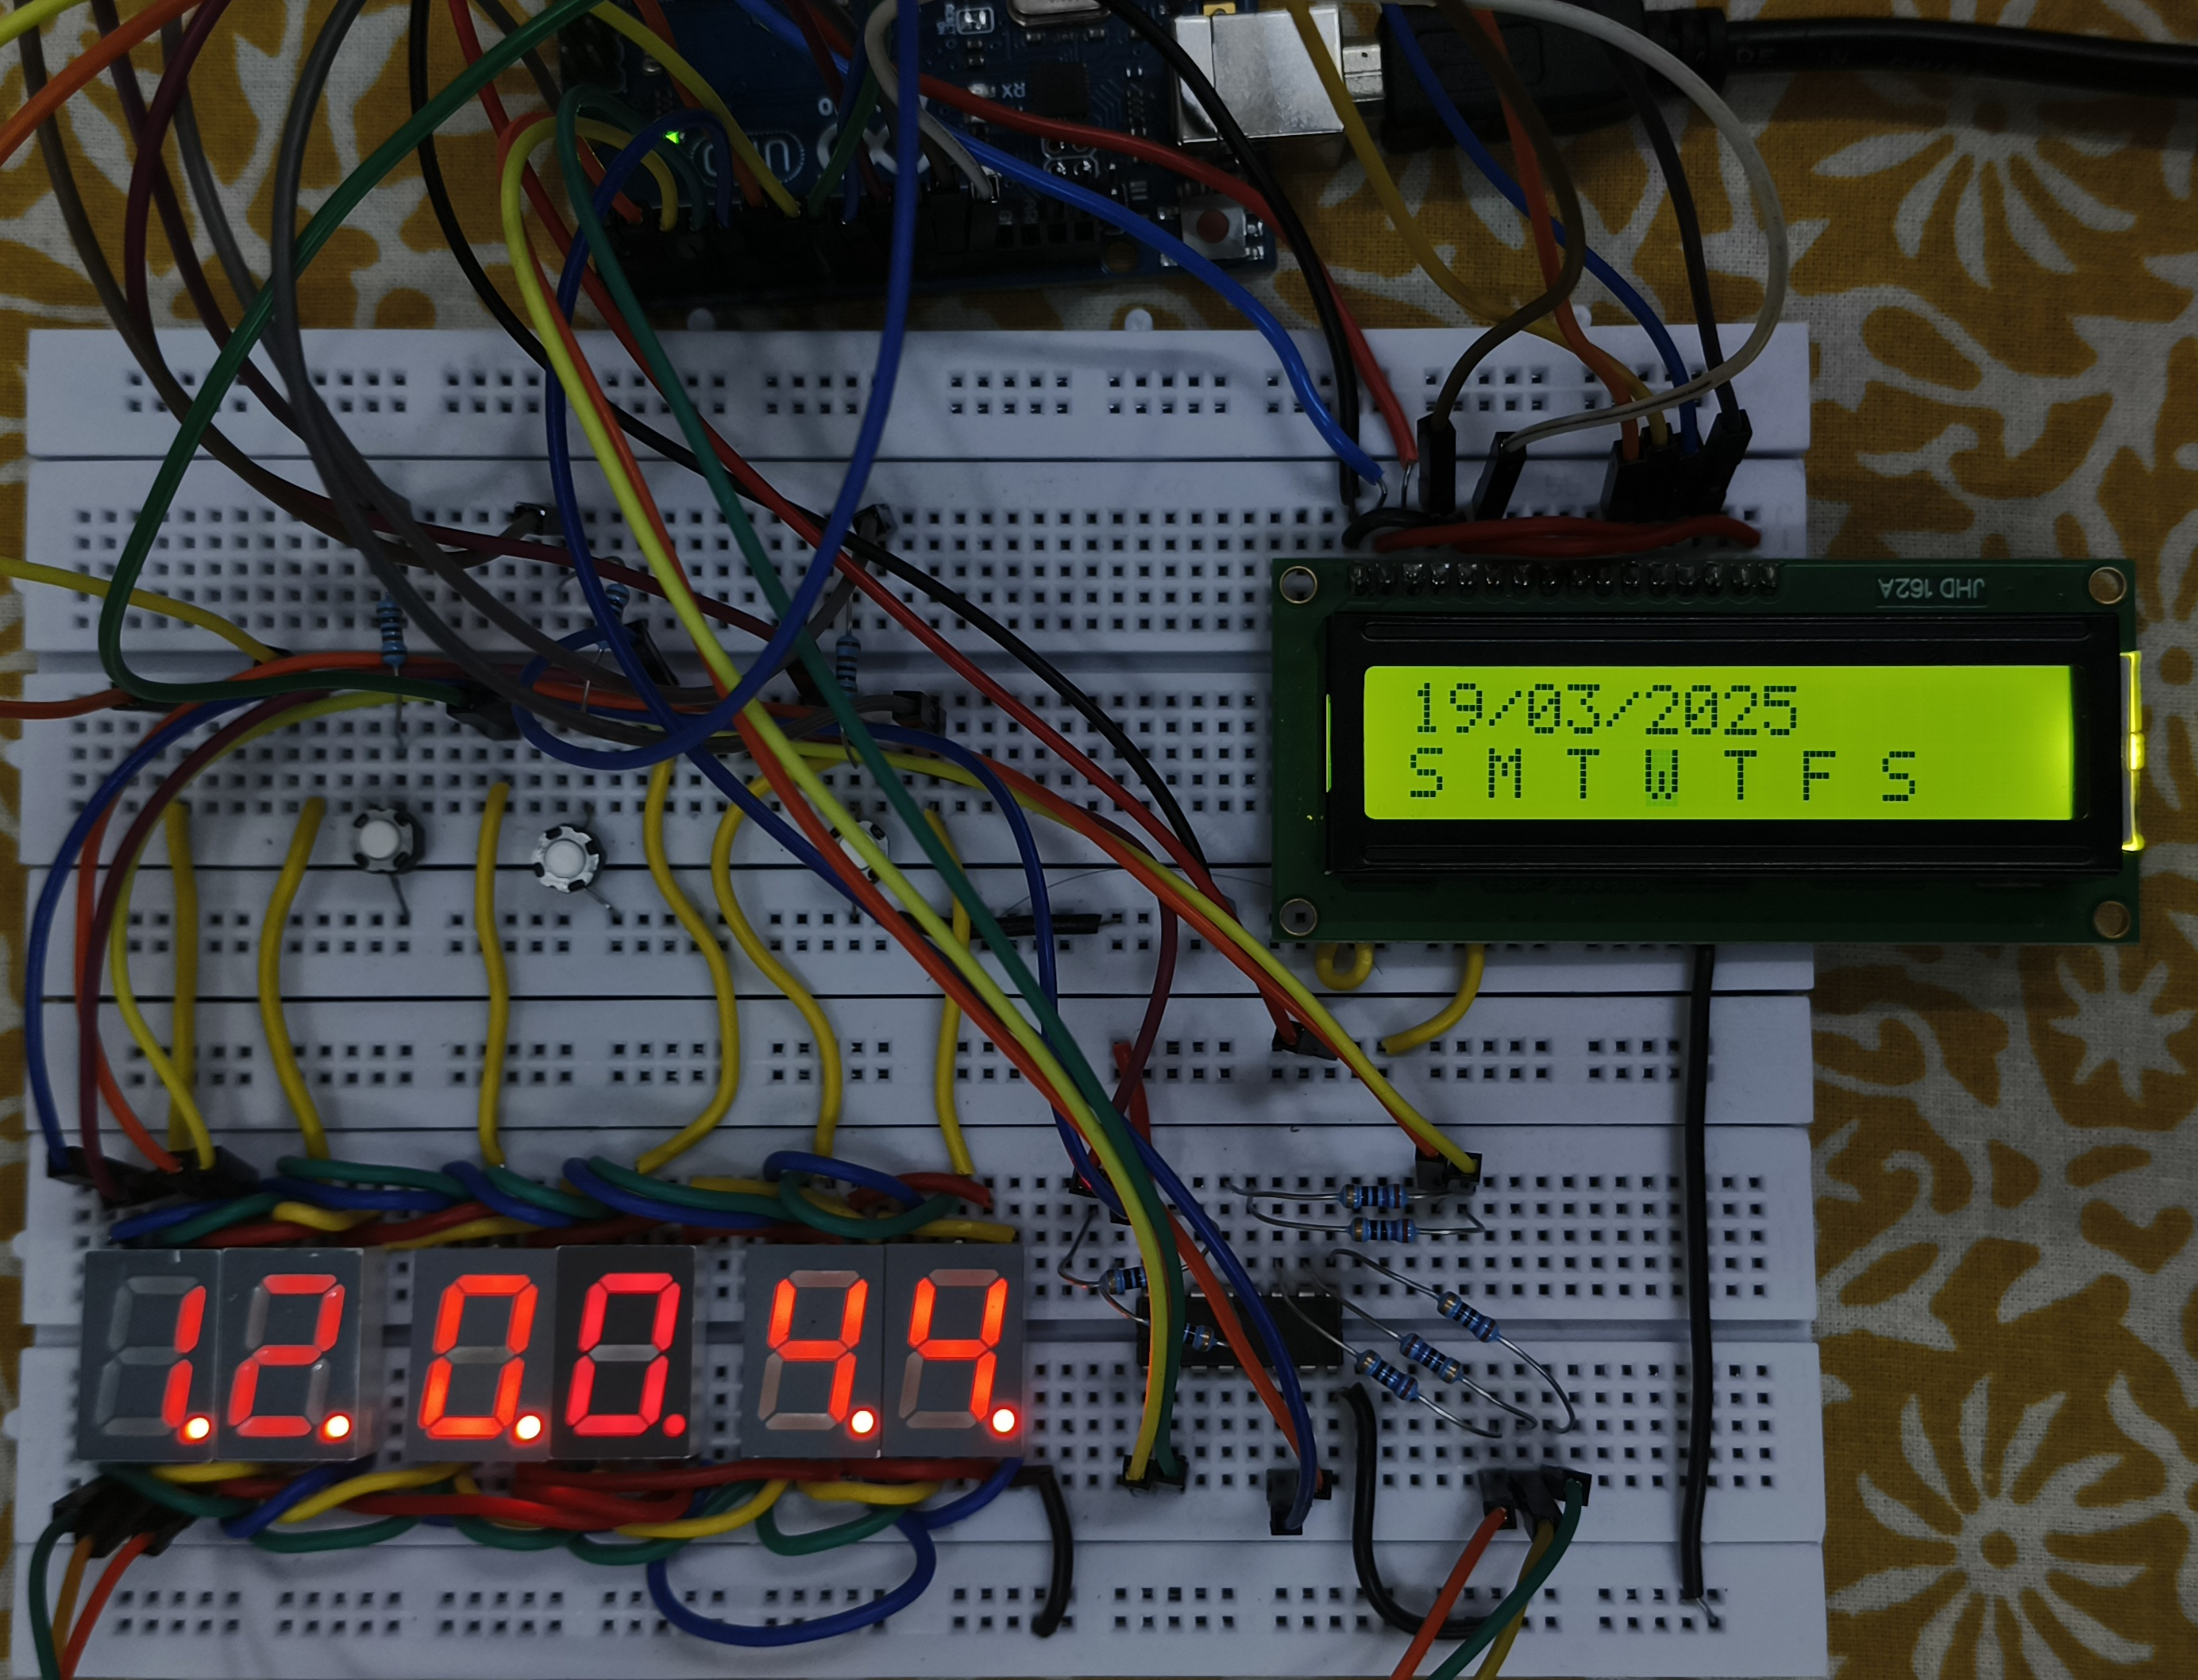
\includegraphics[width=0.5\textwidth]{figs/1.jpg}
    \end{center}
		\begin{center}
        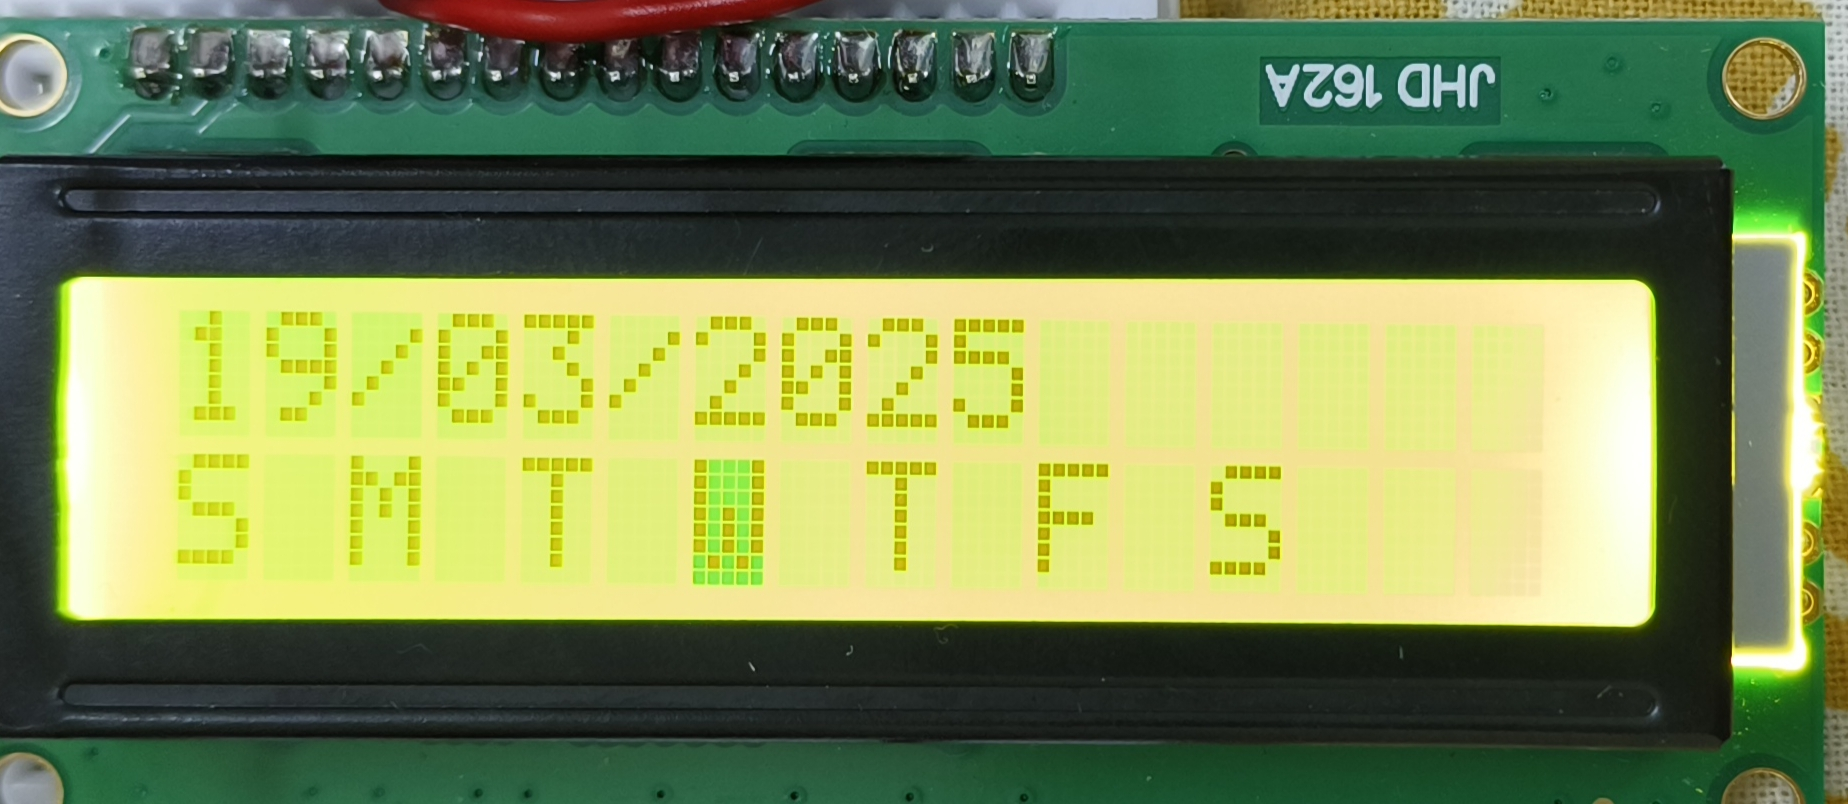
\includegraphics[width=0.5\textwidth]{figs/4.jpg}
    \end{center}
\end{itemize}

\subsection{Stopwatch Mode}
\begin{itemize}
    \item \textbf{Functionality}:
    \begin{itemize}
        \item Starts immediately when Button 2 is pressed
        \item Displays elapsed time in HH:MM:SS
        \item No pause function (requires reset to restart)
    \end{itemize}
    \item \textbf{Image}:
    \begin{center}
        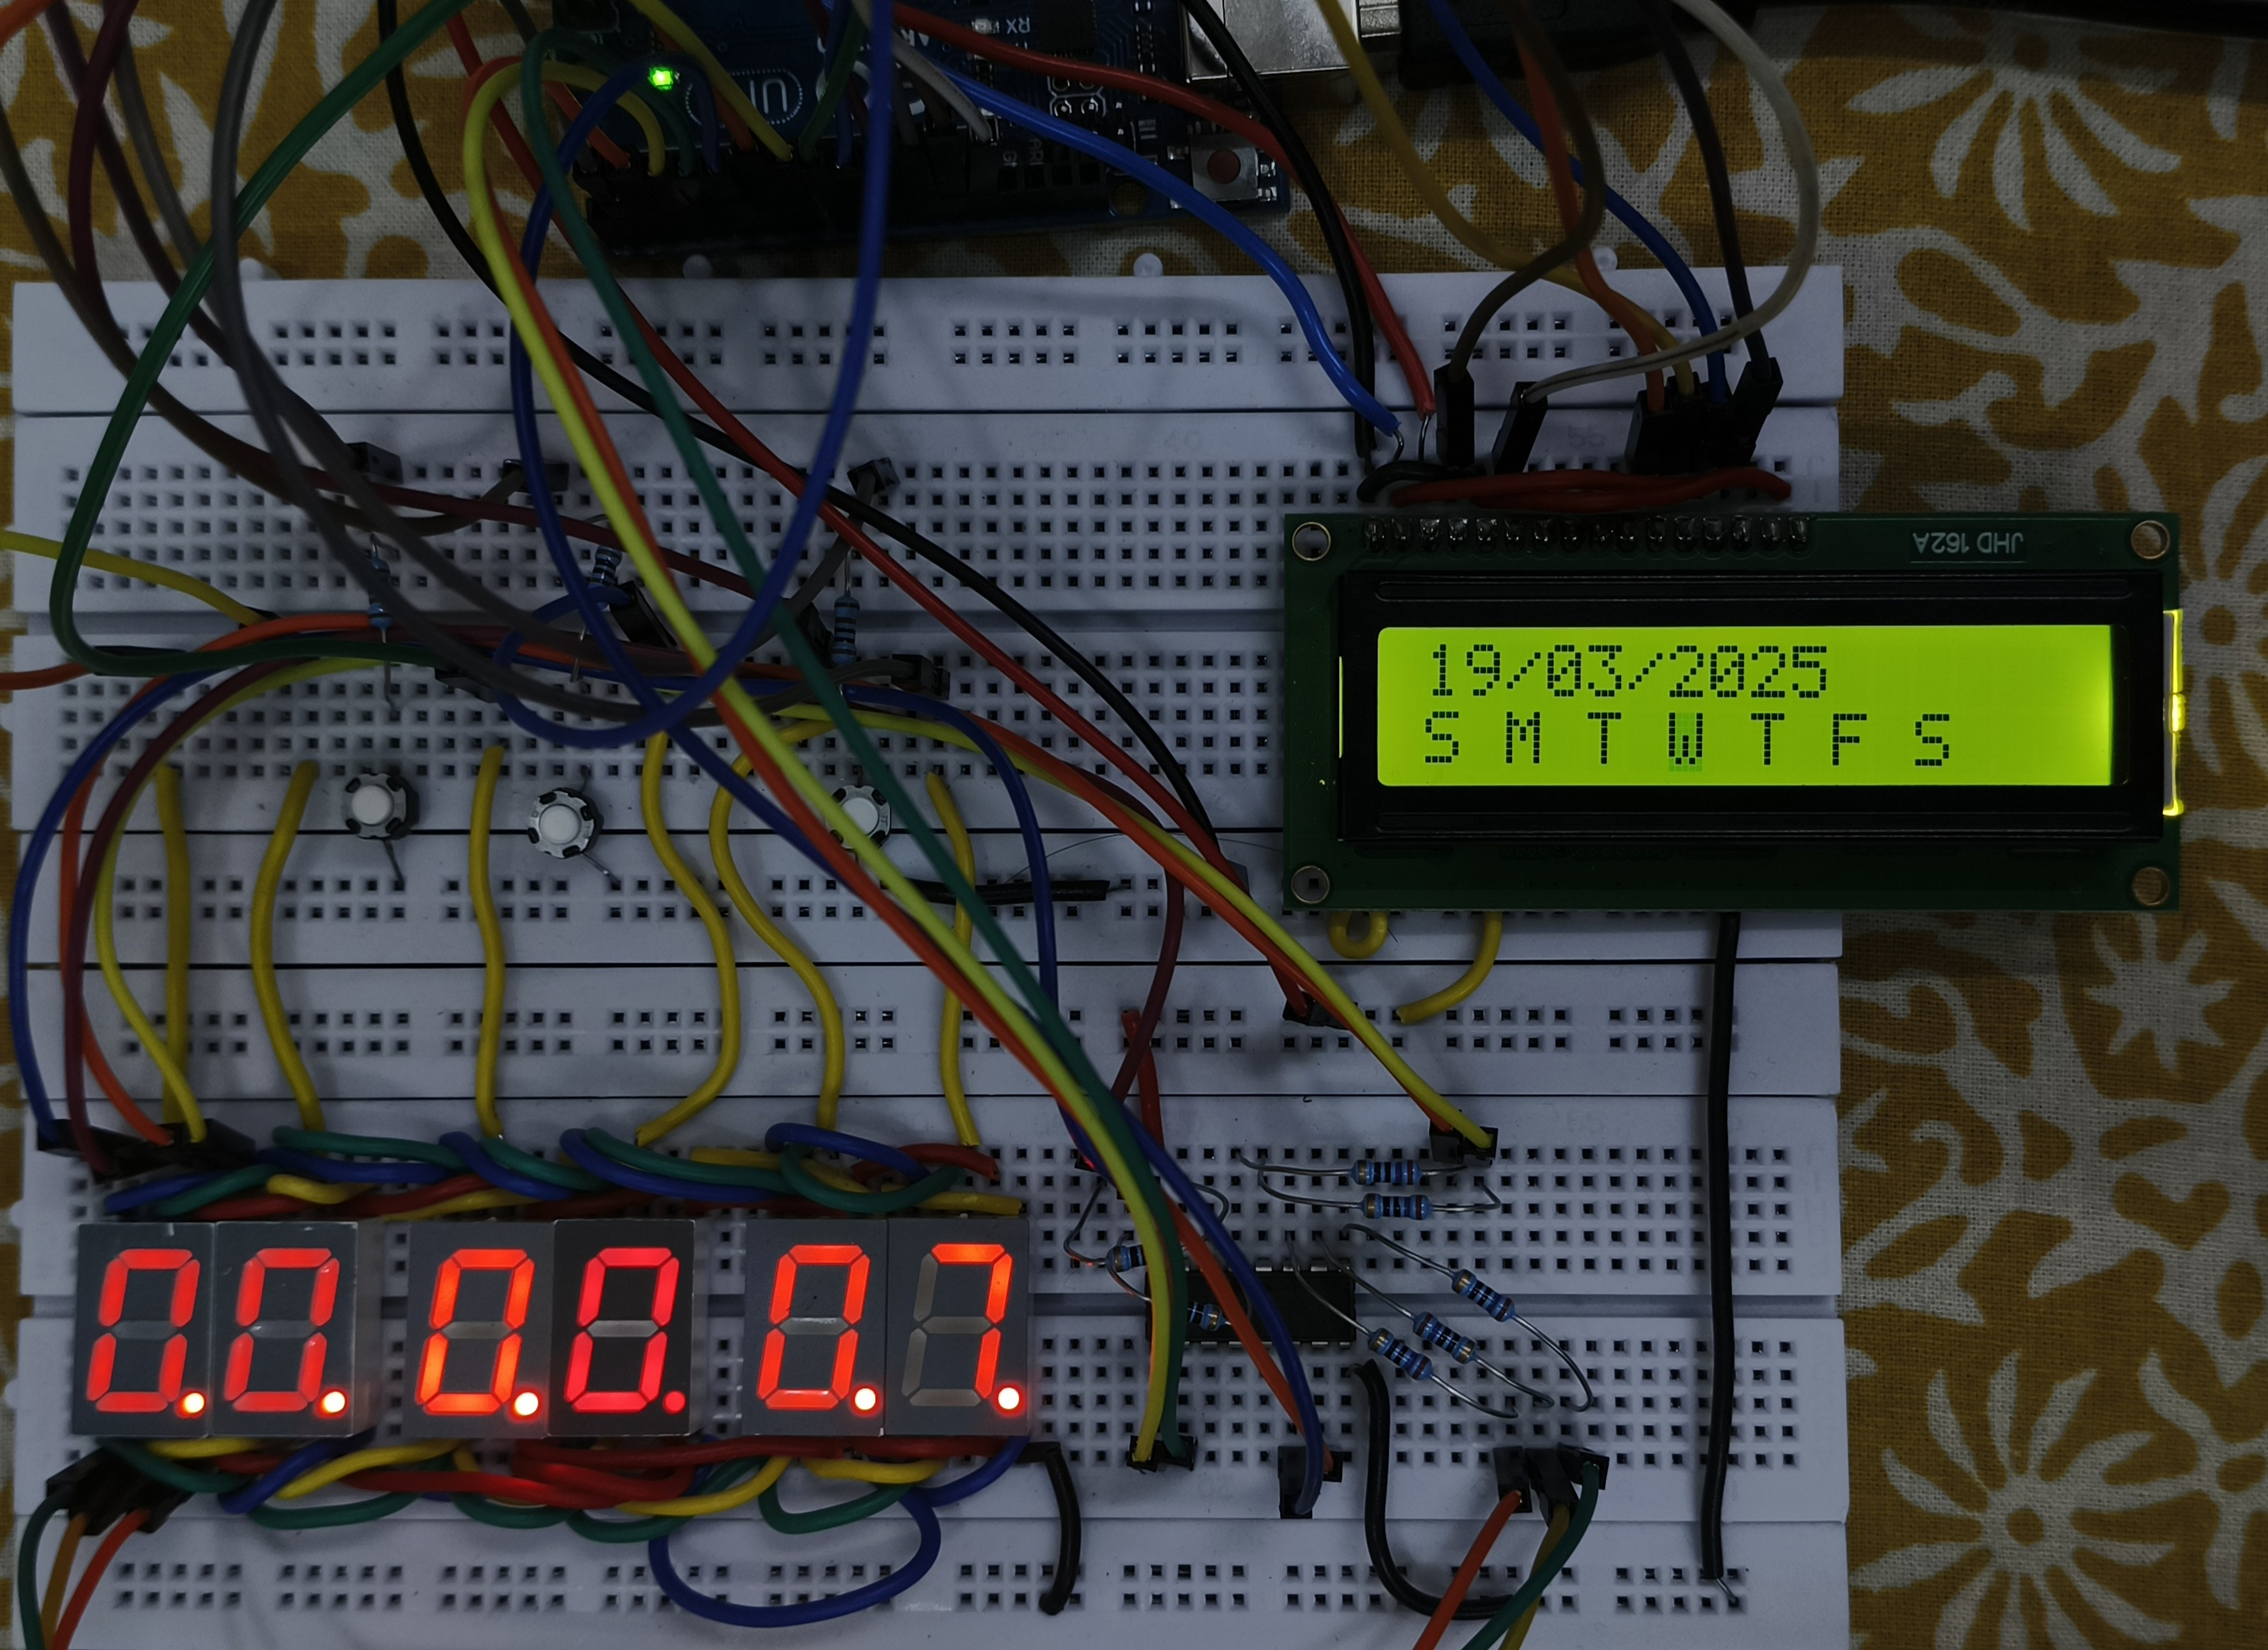
\includegraphics[width=0.5\textwidth]{figs/2.jpg}
    \end{center}
\end{itemize}

\subsection{Timer Mode}
\begin{itemize}
    \item \textbf{Functionality}:
    \begin{itemize}
        \item Starts countdown from preset value (5:00) when Button 3 is pressed
        \item Automatically returns to clock mode at 00:00
    \end{itemize}
    \item \textbf{Image}:
    \begin{center}
        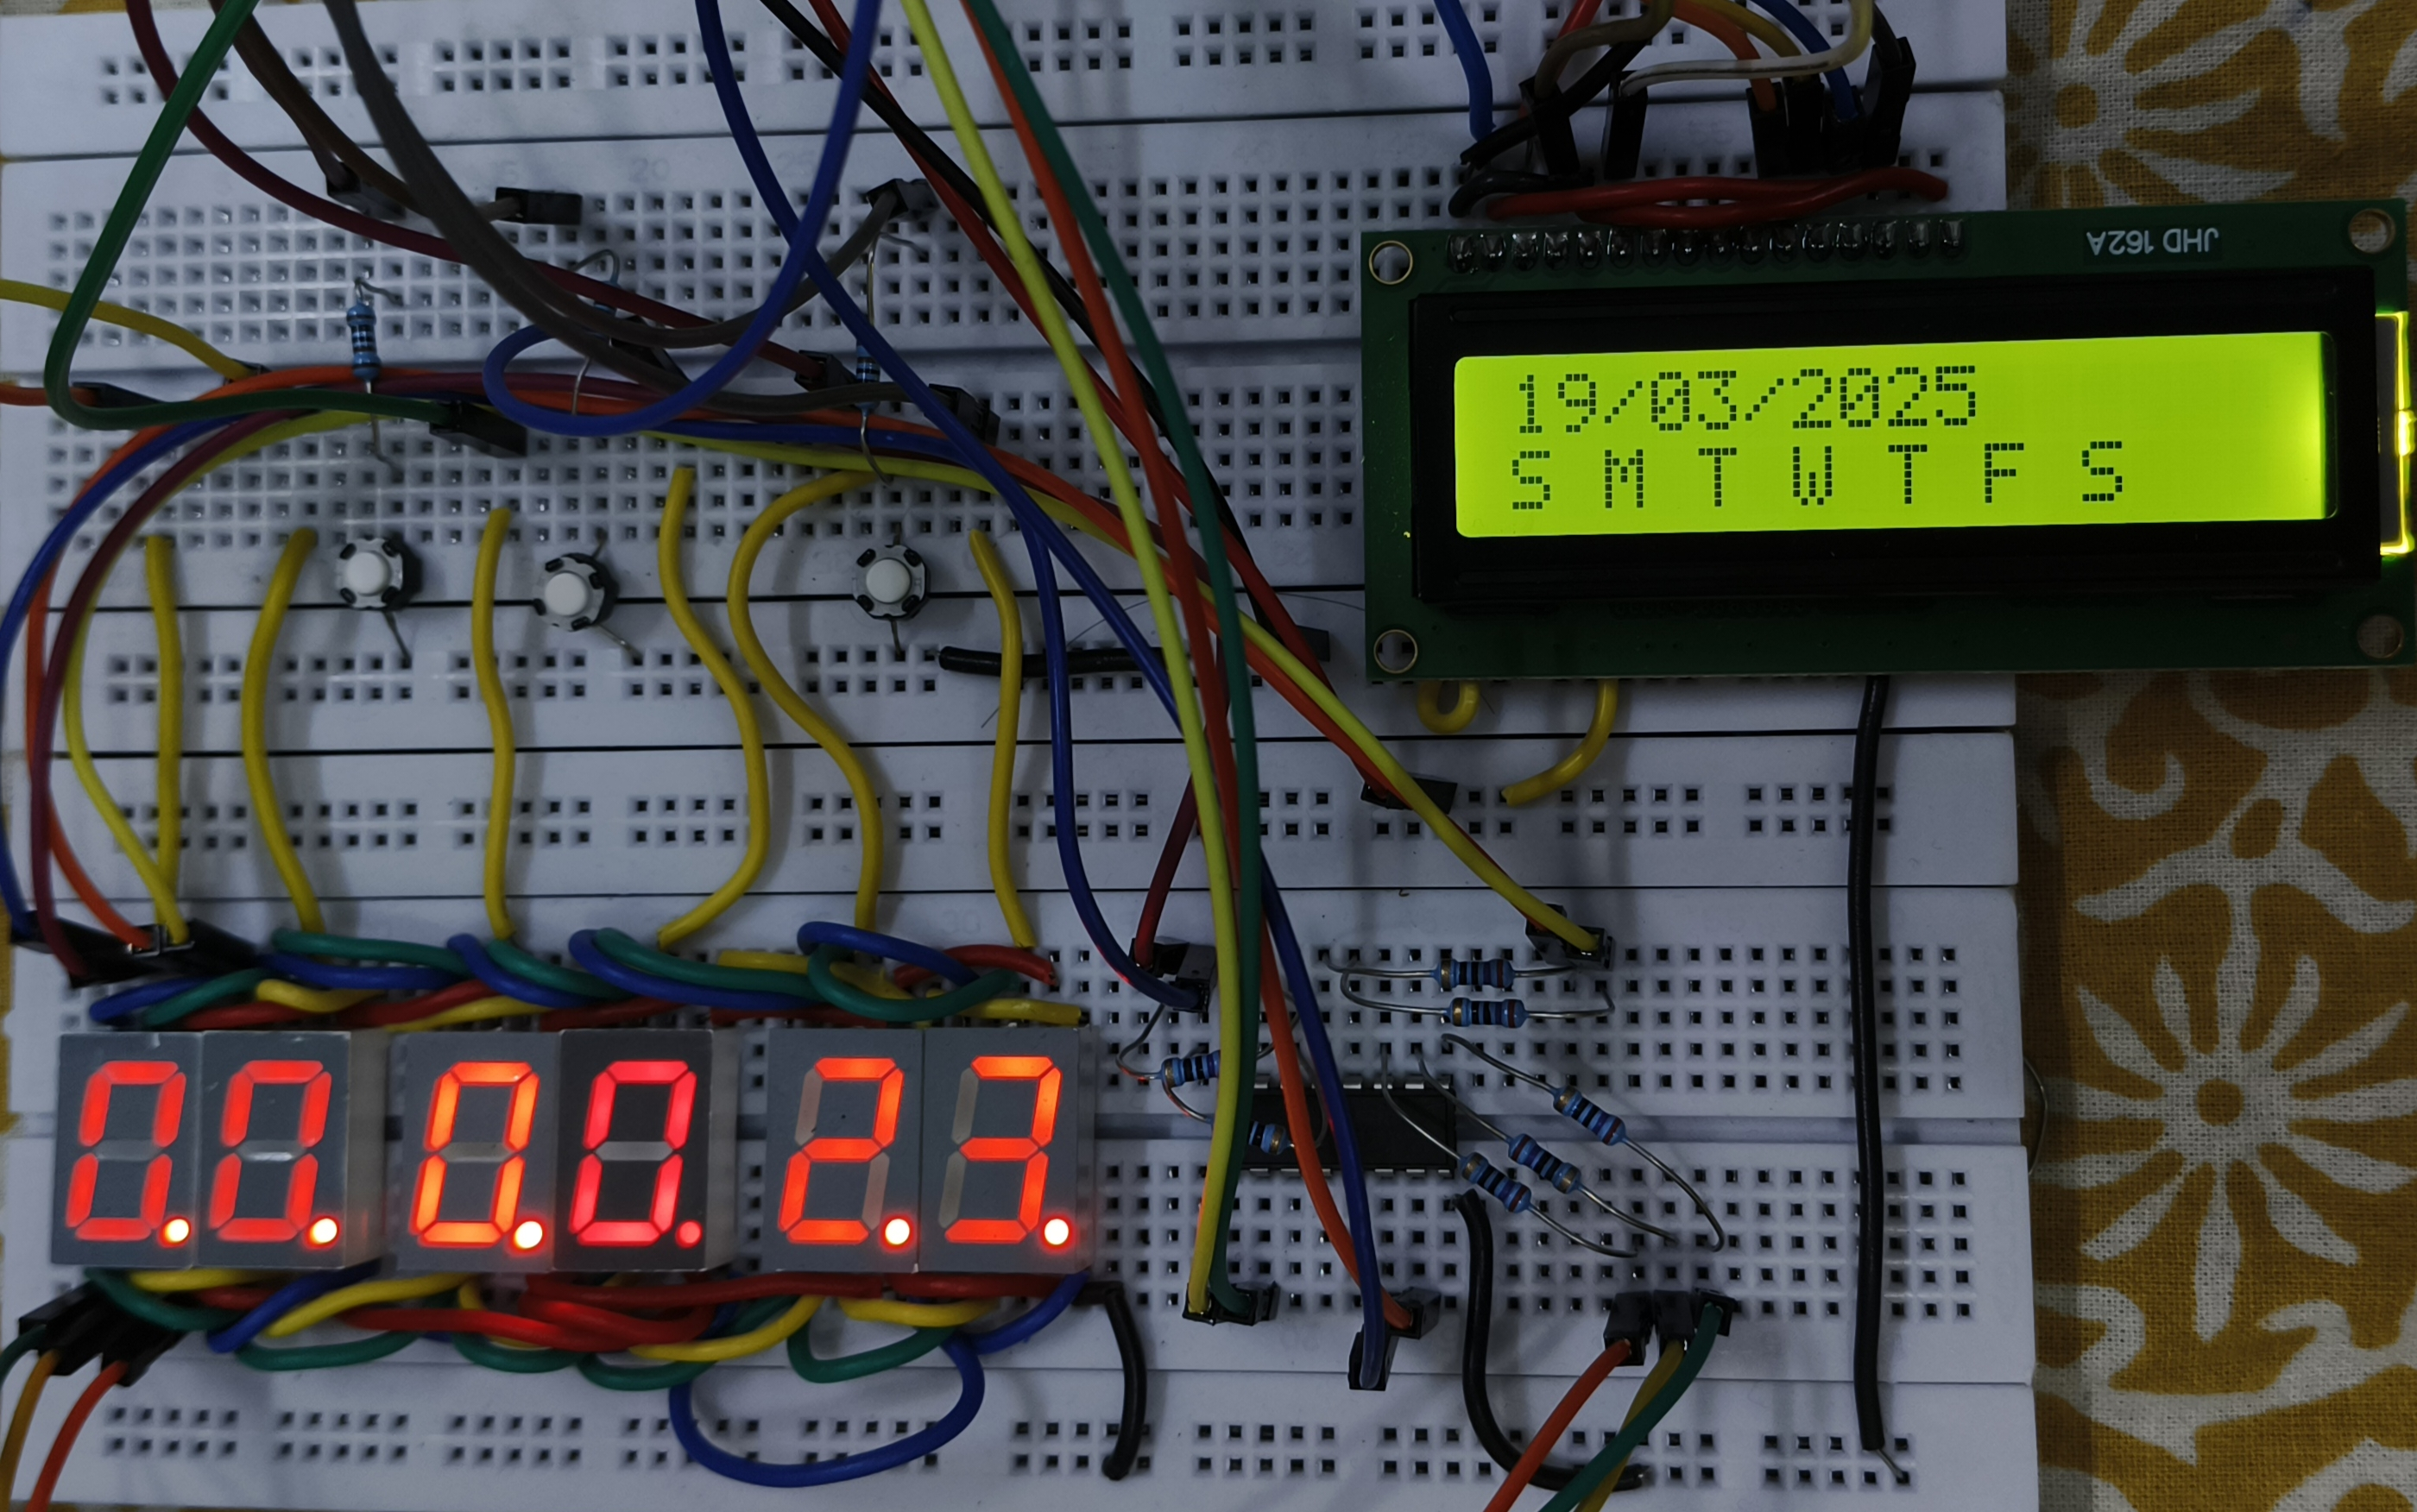
\includegraphics[width=0.5\textwidth]{figs/3.jpg}
    \end{center}
\end{itemize}

\section{Conclusion}
The system successfully implements all required functionalities using only three buttons:
\begin{itemize}
    \item Simplified control scheme (no separate start/stop buttons)
    \item Accurate timekeeping with 1-second resolution
    \item Clear visual feedback through 7-segment displays and LCD
\end{itemize}


\end{document}
